\documentclass[conference]{IEEEtran}
\usepackage[T1]{fontenc}
\usepackage{cite}
\usepackage{amsmath,amssymb}
\usepackage{graphicx}
\usepackage{booktabs}
\usepackage{url}
\usepackage[hidelinks]{hyperref}
\newcommand{\E}{\mathbb{E}}
\newcommand{\KL}{D_{\mathrm{KL}}}
\title{Ego Gate: Evaluating Selective Replay, Online Admission, and Periodic Consolidation}
\author{\IEEEauthorblockN{Aditya Singh}}
\begin{document}
\maketitle

\begin{abstract}
Continual learners must acquire new knowledge while retaining earlier competence under limited memory and computation. We present Ego Gate, a framework separating observation valuation, memory admission, and consolidation, and evaluate offline and online implementations across three studies. An archived Split-Digits study finds that entropy-plus-gradient selection reduces forgetting by 39.4\% relative to random storage across 20 paired seeds. An independent Kaggle reproduction confirms the direction, with a 40.1\% reduction. A subsequent 200-run study evaluates single-pass streams on Digits and Fashion-MNIST, with five seeds, clean and corrupted labels, and ten storage/admission/scheduling conditions. The tested streaming extension does not inherit the offline benefit: on clean Fashion-MNIST, reservoir replay achieves 72.44\% final accuracy versus 29.66\% for the combined score. None of eight specified admission or scheduling contrasts is significant after Holm correction. We distinguish Bayesian information gain from supervised gradient magnitude, identify an intrinsic retention limit of unconditional exploratory replacement, and report resource-accounting and evaluation limitations. The evidence supports a small offline storage result while exposing failures of the particular online extension. An additional 870-run GPU study expands offline selection to randomized task partitions, three memory budgets, and full Fashion-MNIST and CIFAR-10 datasets. Across 27 primary contrasts, EgoGate has no significant wins and ten significant losses after Holm correction. The evidence supports a narrow reproduced result and demonstrates substantial limits to its generalization, rather than validating a general learning controller.
\end{abstract}
\begin{IEEEkeywords}
continual learning, experience replay, memory admission, uncertainty, information gain, adaptive agents
\end{IEEEkeywords}

\section{Introduction}
An intelligent system deployed in a changing environment needs ways to incorporate new evidence while preserving previously useful behavior. Updating model parameters on a non-stationary stream can interfere with earlier representations, whereas a permanently frozen model cannot revise its parameters when the world changes. External retrieval can mitigate outdated information, but introduces its own decisions about which observations to retain, trust, supersede, and retrieve. Both settings motivate a common question: which experiences should influence the system's future behavior?

Ego Gate addresses this question through an explicit control layer between experience and durable learning. The conceptual architecture evaluates observations, retains selected experiences in bounded memory, requests verification when evidence is inadequate, and schedules consolidation. The names \emph{Doubt}, \emph{Curiosity}, \emph{Arrogance}, and \emph{Dreaming} describe uncertainty, model-change estimation, rejection, and replay, respectively. They are organizing metaphors, not evidence of consciousness or a validated psychological taxonomy.

The motivating vision is developmental: retained experience changes the learner, and the changed learner subsequently values experience differently. A further extension would adapt the valuation policy itself. This feedback suggests a research program in learning control, and our experiments test both replay-buffer construction and a specific streaming extension. We preserve that distinction throughout the paper.

Continual learning already includes regularization, architectural methods, and rehearsal. Elastic Weight Consolidation (EWC) protects parameters important to prior tasks \cite{ewc}; replay reduces interference by revisiting earlier examples \cite{robins}. Sample selection is also an established research problem \cite{gss,mir,gcr,grasp}. Thus, neither uncertainty nor selective replay is claimed as new. The contribution is a reproducible initial test within an explicit admission-and-consolidation framework.

Our contributions are fourfold: (1) a resource-constrained formulation that distinguishes these decisions; (2) a precise account of the uncertainty and gradient signals, including their limitations; (3) an audited analysis of a fixed-memory, fixed-replay-exposure study with paired inference; and (4) a completed streaming evaluation that reveals where a particular extension fails. An additional 870-run offline evaluation tests randomized partitions, multiple memory budgets, and two larger image datasets, revealing limits of the original selector itself. The manuscript does not claim that the complete controller, an agent-memory product, or an AGI-scale learner has been validated.

\section{Related Work and Scope}
\subsection{Continual Learning and Replay}
Rehearsal and pseudorehearsal address interference by maintaining access to earlier distributions \cite{robins}. EWC instead uses a parameter-importance penalty \cite{ewc}. These mechanisms can be combined with admission policies: storage determines available evidence, retrieval determines the evidence used in an update, and optimization determines the resulting parameter movement.

Gradient-based Sample Selection (GSS) uses gradient-space diversity to construct a replay buffer \cite{gss}. Maximally Interfered Retrieval (MIR) selects stored examples expected to suffer from an upcoming update \cite{mir}. Gradient Coreset Replay (GCR) approximates historical gradients with selected examples \cite{gcr}. GRASP studies a replay curriculum that progresses from prototypical toward harder examples under compute constraints \cite{grasp}. These works preclude a broad novelty claim that replay methods previously lacked principled selection. They also motivate controls beyond random storage.

\subsection{Uncertainty and Information Gain}
Predictive entropy expresses uncertainty in a predictive distribution, but does not by itself separate epistemic uncertainty from observation noise \cite{kendall}. Calibration can improve agreement between confidence and empirical accuracy \cite{guo}; it does not make confident errors impossible or isolate uncertainty reducible through learning. Bayesian approximations such as MC Dropout provide alternative estimators \cite{gal}.

VIME uses information gain about a dynamics model as an intrinsic exploration reward \cite{vime}. Ego Gate's Bayesian motivation is related, but its present deterministic implementation has no explicit posterior over parameters. A gradient-norm score should therefore be described as a supervised influence heuristic rather than as an exact information-gain estimator.

\subsection{Biological and Developmental Motivation}
Complementary learning systems theory motivates separating rapid experience storage from slower integration \cite{cls}. It does not imply that arbitrary offline replay preserves all old knowledge. Consolidation still depends on representative memory, optimization, capacity, and the data distribution.

Similarly, recursive synthetic-data training can degrade learned distributions \cite{collapse}, but a frozen network does not decay merely because no stimulus arrives. Staleness, recursive distributional degradation, and catastrophic forgetting are distinct problems. The current classification study measures only the last of these. Continual learning is a candidate ingredient in more general intelligence, not a sufficient definition or demonstrated route to it.

\section{A Resource-Constrained Control Formulation}
Let $o_t=(x_t,y_t,m_t)$ denote an observation, an optional label, and provenance metadata. The learner has parameters $\theta_t$, persistent memory $B_t$, a temporary consolidation queue $Q_t$, and controller state $\phi_t$. A policy chooses an action
\begin{equation}
 a_t\sim\pi_{\phi_t}(a\mid o_t,\theta_t,B_t,Q_t),
\end{equation}
from rejection, retention, verification, or immediate update. A separate scheduling decision determines whether to consolidate queued experiences. This decomposition avoids treating every high score as an immediate weight update.

A long-horizon design objective is
\begin{align}
\max_{\pi}\quad &\E\!\left[\sum_t\gamma^t\{\Delta U_t-\lambda_h H_t-\lambda_c C_t\}\right] \\
\text{subject to}\quad & |B_t|+|Q_t|\le M,\quad
\sum_t C_t\le C_{\max},\\
&N_{\mathrm{verify}}\le V_{\max}.
\end{align}
Here $\Delta U_t$ denotes improvement in future task utility, $H_t$ denotes harm to previously useful competence, and $C_t$ includes valuation, retrieval, verification, and optimization costs. These are design quantities rather than observables supplied by the current benchmark. In particular, a sample's future utility is generally unknown at admission time. Estimating it from delayed feedback is the central control problem; writing this objective does not solve it.

Memory budgets must include temporary queues, labels, and metadata. Equal update counts alone do not imply equal compute, because one policy may perform additional forward passes or gradient calculations. Experiments must report these costs separately and, when possible, compare performance under a total wall-time or measured-operation budget.

\subsection{Doubt}
For a $K$-class model, define normalized predictive entropy
\begin{equation}
 D_t=-\frac{1}{\log K}\sum_{c=1}^K p_\theta(c\mid x_t)\log p_\theta(c\mid x_t).
\end{equation}
Then $D_t\in[0,1]$. High entropy can identify unfamiliar decision regions, but can also reflect class overlap or corrupted observations. Conversely, a confident error can receive a low score. An ensemble disagreement estimator could address some of these limitations, at additional cost; no such estimator is used in the archived experiment.

\subsection{Curiosity: Three Different Quantities}
For a Bayesian learner, realized belief revision after a labeled observation is
\begin{equation}
 C_t^{\mathrm{Bayes}}=\KL\big(q(\theta\mid\mathcal D_t\cup\{(x_t,y_t)\})
 \Vert q(\theta\mid\mathcal D_t)\big).
\end{equation}
Before acquiring $y_t$, an expected information-gain score must integrate over possible outcomes. Conditioning a supervised posterior on $x_t$ alone silently changes the problem and is not justified by the present implementation.

For deterministic parameters, a different quantity measures local change in predictive distributions. With an explicitly chosen reference input distribution $\mu$,
\begin{align}
 \E_{x\sim\mu}\KL(p_{\theta+\delta}(\cdot\mid x)\Vert p_\theta(\cdot\mid x))
 &\approx\tfrac12\delta^T F_\mu(\theta)\delta,\\
 \delta=-\eta g_t\quad\Longrightarrow\quad C_t^{\mathrm{local}}
 &\approx\tfrac{\eta^2}{2}g_t^T F_\mu(\theta)g_t.
\end{align}
This Fisher-metric expansion concerns predictive change, not a posterior over weights \cite{amari}. Replacing $F_\mu$ with the identity yields a squared gradient norm. It discards the geometry and is sensitive to parameterization. Neither this replacement nor a more accurate Fisher approximation guarantees better downstream retention.

For the experimental network, let $h=\operatorname{ReLU}(W_1x+b_1)$, $p=\operatorname{softmax}(W_2h+b_2)$, $e=p-\operatorname{onehot}(y)$, and $u=(W_2^Te)\odot\mathbf1_{h>0}$. Cross-entropy gives the exact identity
\begin{equation}
 \label{eq:gradient}G(x,y)=\|\nabla_\theta\ell\|_2^2
 =\|e\|_2^2(\|h\|_2^2+1)+\|u\|_2^2(\|x\|_2^2+1).
\end{equation}
The bias terms account for the two $+1$ factors. This analytic implementation avoids materializing a gradient tensor for every example, but remains label-dependent and computationally more expensive than entropy alone. Large $G$ denotes potential movement, not necessarily beneficial learning.

\subsection{Valuation, Reliability, and Exploration}
The archived experiment uses
\begin{equation}
 \label{eq:offline}V(x,y)=z(D(x))+z(G(x,y)),
\end{equation}
where each $z$-score is calculated over the available Task-A training pool at a frozen checkpoint. This is legitimate for offline storage selection, but cannot be transferred unchanged to a future-unknown stream.

A conceptual routing rule should give verification precedence:
\begin{equation}
a_t=\begin{cases}
\mathrm{verify},&r_t<r_{\min},\\
\mathrm{retain},&r_t\ge r_{\min}\ \land\ V_t\ge\tau_t,\\
\mathrm{reject},&\text{otherwise},
\end{cases}
\end{equation}
where $r_t$ is a separately estimated reliability signal. Entropy is not used as a synonym for reliability or poisoning detection. Estimating $r_t$ and adapting $\tau_t$ are open components, not validated mechanisms in this paper.

Permanent rejection based solely on current confidence can reinforce existing errors. An exploratory bypass can admit some otherwise rejected observations with probability $\epsilon$. For $n$ independent bypass trials, the probability of no bypass is $(1-\epsilon)^n$. This elementary observation concerns opportunities for admission only; it guarantees neither retention nor useful learning after admission.

\section{Memory and Consolidation}
\subsection{Separation of Decisions}
Storage selection chooses what remains available. Replay retrieval chooses what is used in a specific update. Admission determines whether a new observation can directly contribute a training gradient. Consolidation determines when updates occur. A study changing several of these simultaneously cannot attribute an improvement to a particular component without ablations.

For selected recent observations $Q$ and historical memory $B$, a consolidation objective is
\begin{equation}
 \mathcal L_{\mathrm{con}}(\theta)=\E_{(x,y)\sim Q}\ell_\theta(x,y)
 +\lambda\E_{(x,y)\sim B}\ell_\theta(x,y).
\end{equation}
The coefficient $\lambda$ expresses a stability preference, but does not guarantee a stability level. A bounded memory cannot preserve arbitrary historical detail. A practical controller should consider coverage and rare examples as well as difficulty, and should expose retained provenance and deletion decisions when external memory is involved.

\subsection{An Executable Streaming Extension}
We specify a fixed, task-boundary-agnostic extension evaluated in Section VI. Its combined score is
\begin{equation}
 S_t=\tfrac12\left(D_t+\frac{G_t}{1+G_t}\right).
\end{equation}
The bounded transform removes the need for full-stream normalization, but is a new heuristic rather than an equivalent implementation of (\ref{eq:offline}). Its sensitivity to gradient scale remains a limitation. Comparisons with entropy-only and gradient-only variants are therefore required.

When memory is full, the controller samples one stored candidate uniformly and rescoring compares it with the arriving example under the current parameters. The higher-score example is retained, with an optional $\epsilon$ bypass for the incoming observation. This avoids indefinitely comparing stale stored scores with fresh scores. It is a stochastic replacement heuristic; it is not global top-$K$ selection or a theorem about optimal retention.

In the admission variant, only admitted new observations enter the update queue. Rejected positions in the fixed training budget are replaced with replay samples. This isolates allocation of training exposure while holding update counts and total trained-example exposures constant. It does not claim that rejection saves compute in this protocol. The storage-only variant still trains on all arriving examples and provides the necessary ablation.

The periodic variant accumulates up to eight minibatches before performing the same number of updates. Temporary storage and adaptation delay therefore increase. Task boundaries are used solely by the evaluator; they do not trigger consolidation.

\section{Archived Split-Digits Experiment}
\subsection{Question and Provenance}
The completed study asks whether model-state-aware storage improves retention relative to random storage at an equal buffer size and replay exposure. Numerical results in this section come from the repository's archived per-seed outputs. The present preparation independently recomputes descriptive and paired statistics; it does not represent those archived runs as newly executed Kaggle experiments. A private Kaggle notebook additionally completed an independent reproduction and the streaming extension, reported below.

\subsection{Data and Training}
The scikit-learn Digits dataset contains 1,797 images with 64 input features \cite{digits,sklearn}. Classes 0--4 form Task A; classes 5--9 form Task B. Each task uses a stratified 80/20 train/test split with data seed zero. The ten-output classifier has one 64-unit ReLU hidden layer. SGD uses learning rate 0.5 and minibatch size 32. Task A is trained for 60 epochs; Task B for 40 epochs. All conditions within a seed begin at the same Task-A checkpoint.

After Task-A training, selectors score the 720 Task-A training examples and retain 40. During Task-B learning, each new-task minibatch receives two uniformly sampled replay examples, and a single cross-entropy loss is averaged over the combined batch. FullMemory stores all 720 earlier examples but receives the same two replay samples per update. Thus, it tests broader replay access rather than a larger update budget. NoReplay is a diagnostic lower control, not a matched-replay-compute condition.

The conditions are random storage; class-balanced random storage; entropy-only Doubt; gradient-only Curiosity; their equally weighted standardized combination; embedding k-center; k-center within a top-$5K$ EgoGate candidate pool; full memory; and no replay. The diversity variants use standardized hidden features. None of these conditions filters incoming Task-B training examples or schedules a distinct offline consolidation phase.

\subsection{Metrics and Statistical Analysis}
Forgetting is the difference between Task-A test accuracy immediately before and after learning Task B. Task-B accuracy measures new-task performance. Twenty training seeds vary initialization and training randomness, while the train/test split is fixed. These repetitions estimate conditional variability on one split, not generalization across independently sampled datasets.

Paired comparisons align seeds. The analysis reports a paired $t$ statistic, Cohen's $d_z$ (mean paired improvement divided by its sample standard deviation), and a 95\% $t$ interval. Holm correction \cite{holm} is applied across the eleven comparisons generated by the archived analysis: eight conditions versus random and three component/diversity comparisons versus EgoGate. This is the available comparison family, not a claim of preregistration. Hyperparameter-selection history is not recorded sufficiently to exclude all exploratory selection effects.

\begin{table*}[t]
\caption{Archived Split-Digits results across 20 paired training seeds. Entries are mean $\pm$ sample standard deviation in percentage points. Higher accuracy and lower forgetting are better. Full memory has a larger storage budget; no replay has no replay exposure.}
\label{tab:results}
\centering\small
\begin{tabular}{lrrrr}
\toprule
Storage policy & Stored examples & Task-A final accuracy & Forgetting & Task-B final accuracy\\
\midrule
% BEGIN GENERATED TABLE
No replay & 0 & 0.00 $\pm$ 0.00 & 99.45 $\pm$ 0.00 & 99.81 $\pm$ 0.33 \\
Random & 40 & 80.17 $\pm$ 3.21 & 19.28 $\pm$ 3.21 & 99.08 $\pm$ 0.81 \\
Balanced random & 40 & 82.68 $\pm$ 3.28 & 16.77 $\pm$ 3.28 & 98.97 $\pm$ 1.12 \\
Embedding k-center & 40 & 84.09 $\pm$ 4.74 & 15.36 $\pm$ 4.74 & 98.94 $\pm$ 1.25 \\
Curiosity & 40 & 87.62 $\pm$ 4.33 & 11.82 $\pm$ 4.33 & 99.25 $\pm$ 0.68 \\
EgoGate & 40 & 87.76 $\pm$ 4.51 & 11.69 $\pm$ 4.51 & 99.03 $\pm$ 1.02 \\
EgoGate + diversity & 40 & 86.38 $\pm$ 2.68 & 13.07 $\pm$ 2.68 & 98.61 $\pm$ 2.03 \\
Doubt & 40 & 89.20 $\pm$ 4.16 & 10.25 $\pm$ 4.16 & 98.50 $\pm$ 1.79 \\
Full memory & 720 & 93.51 $\pm$ 1.70 & 5.94 $\pm$ 1.70 & 97.72 $\pm$ 3.38 \\
% END GENERATED TABLE
\bottomrule
\end{tabular}
\end{table*}

\begin{figure*}[t]
\centering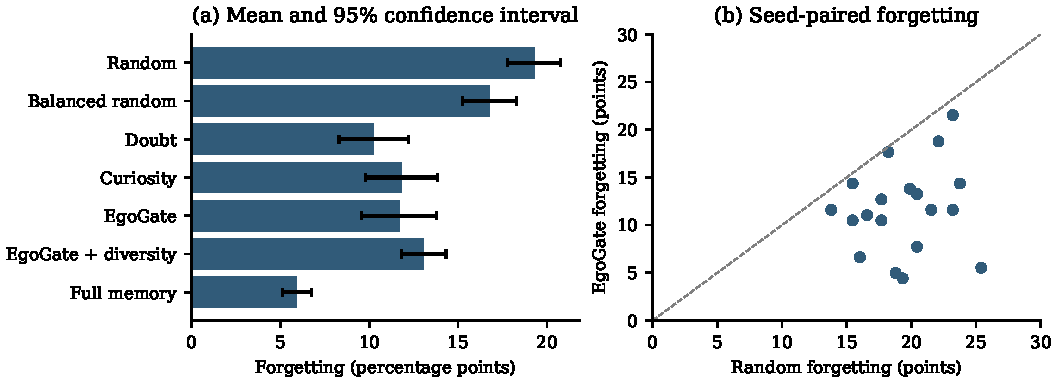
\includegraphics[width=\textwidth]{retention.pdf}
\caption{Archived evidence. (a) Forgetting with confidence intervals over training seeds on the fixed data split; these are not prediction intervals across new datasets. (b) Seed-aligned random and EgoGate forgetting. The diagonal denotes equal forgetting.}
\label{fig:retention}
\end{figure*}

\subsection{Results}
Table~\ref{tab:results} reports all archived conditions. EgoGate reduces mean forgetting from 19.28 to 11.69 points. The paired reduction is 7.60 points, with 95\% interval [5.20, 9.99]; the relative reduction is 39.4\%. The paired statistic is $t(19)=6.64$, unadjusted $p=2.35\times10^{-6}$, Holm-adjusted $p=1.41\times10^{-5}$, and $d_z=1.49$. Figure~\ref{fig:retention} shows both aggregate and paired observations.

Doubt has the lowest bounded-buffer mean forgetting, 10.25 points. Its paired advantage over EgoGate is 1.44 points, with unadjusted $p=0.048$ and Holm-adjusted $p=0.144$. This does not establish a difference after correction, and it is not an equivalence test. The evidence therefore supports informed storage relative to random selection, but does not establish that adding Curiosity improves Doubt.

Class-balanced random storage improves mean retention relative to unconstrained random storage, while diversity-constrained EgoGate does not improve the combined selector's mean. These observations caution against assuming that any diversity mechanism is automatically beneficial. FullMemory achieves the strongest old-task retention, with lower and more variable Task-B accuracy. Retention must therefore be interpreted alongside acquisition of new competence.

\subsection{What the Result Does Not Show}
The experiment contains one small dataset, one architecture, one task transition, and one memory/replay configuration. It lacks measured total selection cost, repeated data splits, strong published selector implementations, and a held-out policy-selection protocol. It cannot establish online admission benefits, label-noise robustness, poisoning detection, schedule superiority, or general-purpose agent learning.

\section{Kaggle Streaming Evaluation}
The accompanying notebook fixed the following protocol before execution. All 200 condition-seed runs completed on Kaggle, and downloaded raw trajectories passed checks for unique conditions, matched update/exposure budgets, buffer size, and five evaluation checkpoints. Digits and Fashion-MNIST \cite{fashion} are partitioned into five two-class phases with seed-dependent class ordering. The learner receives one pass through training examples, a fixed ten-class output head, and no task identifier. Evaluation boundaries can fall inside a minibatch; the evaluator records the actual observation count. This is a class-incremental stream with hidden boundaries, not a fully naturalistic task-free environment.

The executed protocol uses five seeds, clean and 20\% symmetric label corruption, a 200-example persistent buffer, a 128-unit ReLU hidden layer, batch size 32, and SGD learning rate 0.05. Digits uses seed-dependent stratified splits; Fashion-MNIST uses its official train/test split. Corruption affects training labels only, and incorrect replacements are sampled from the other nine classes. The gate never receives the corruption indicator; it is retained solely for diagnostic reporting.

Six immediate, storage-only selectors are compared: reservoir sampling, online class-balanced random replacement, Doubt, Curiosity, EgoGate, and EgoGate with a 0.1 exploratory bypass. Four additional conditions isolate periodic replay and actual training admission: periodic reservoir, periodic bypass-EgoGate, immediate admission-EgoGate, and periodic admission-EgoGate. The online balanced baseline is explicitly a random replacement heuristic, not a claim to implement an optimal balanced reservoir.

Every stream minibatch receives one optimization update and the same total trained-example exposure across conditions. In admission conditions, extra replay fills the positions of rejected new examples. The periodic variants delay rather than remove updates. Their queue can hold up to 256 newly admitted examples, versus at most 32 for immediate variants, so equality of persistent buffer size is not equality of total peak sample storage. Both quantities are logged. These counts describe logical learner memory; the experimental data loader also materializes the dataset, so they are not process-RAM measurements.

Primary reporting comprises final average accuracy, forgetting over the first four phases, and mean seen-class accuracy at evaluation checkpoints. Additional diagnostics include admission fraction, retained corruption fraction, scorer calls, scoring wall time, end-to-end wall time, update counts, training exposures, and peak queue size. Wall times include evaluation overhead and are meaningful only alongside hardware and software manifests. Corruption enrichment is a diagnostic, not a poisoning-detection metric.

The primary comparisons are admission-EgoGate versus its storage-only counterpart and periodic versus immediate admission-EgoGate, separately for each dataset/noise regime. Paired inference corrects across this eight-comparison family and reports effect intervals. With five seeds, uncertainty is substantial; absent significance is not evidence of equivalence. Secondary selector comparisons are exploratory. A broader study should add GSS, MIR, GCR, and GRASP with their implementation details and compute costs, then vary memory budgets, stream orders, and optimizer settings using validation data rather than the final test stream.

The notebook writes source hashes, environment information, raw seed-level trajectories, and a completion marker. Partial outputs cannot be described as a completed study. The completion marker and normalized source hashes match the supplied code. The run used CPU execution, Python 3.13.18, PyTorch 2.11.0+cpu, NumPy 2.1.3, SciPy 1.16.3, and scikit-learn 1.6.1. CPU model and torchvision version were not recorded, limiting exact environmental reconstruction.

\subsection{Independent Reproduction}
The Kaggle reproduction contains 180 condition-seed runs. Mean forgetting is 19.28 points for random storage and 11.55 for EgoGate: a 40.1\% relative reduction, paired $t(19)=6.78$, $d_z=1.52$, and Holm-adjusted $p=1.07\times10^{-5}$. Doubt yields 10.39 points; its comparison with EgoGate is not significant (Holm $p=0.365$). Small numerical differences from the archive are retained rather than overwritten. This confirms the qualitative offline finding, not bitwise reproducibility or cross-dataset generality.

\begin{table*}[t]
\caption{Completed streaming study: final mean accuracy (\%) $\pm$ sample standard deviation across five seeds. Noise is the training-label corruption rate. All ten conditions are reported; selectors use the streaming rules, not offline top-$K$ selection.}
\label{tab:stream}\centering\small
\begin{tabular}{lrrrr}\toprule
Condition & Digits, 0\% & Digits, 20\% & Fashion, 0\% & Fashion, 20\%\\\midrule
Reservoir & 49.31 $\pm$ 4.08 & 32.29 $\pm$ 8.31 & 72.44 $\pm$ 3.89 & 69.09 $\pm$ 3.80 \\
Balanced random & 56.12 $\pm$ 3.51 & 39.11 $\pm$ 18.83 & 71.90 $\pm$ 3.73 & 23.07 $\pm$ 4.23 \\
Doubt & 41.24 $\pm$ 4.43 & 39.87 $\pm$ 9.47 & 32.10 $\pm$ 8.16 & 29.94 $\pm$ 5.10 \\
Curiosity & 29.50 $\pm$ 6.62 & 22.70 $\pm$ 8.90 & 29.81 $\pm$ 3.52 & 20.40 $\pm$ 2.81 \\
EgoGate & 27.67 $\pm$ 5.76 & 20.30 $\pm$ 6.11 & 29.66 $\pm$ 5.97 & 31.57 $\pm$ 1.77 \\
EgoGate + bypass & 27.96 $\pm$ 4.89 & 26.80 $\pm$ 6.94 & 20.66 $\pm$ 1.53 & 19.70 $\pm$ 1.02 \\
Reservoir periodic & 55.63 $\pm$ 8.70 & 38.37 $\pm$ 11.15 & 72.83 $\pm$ 3.64 & 69.13 $\pm$ 3.76 \\
Bypass periodic & 22.58 $\pm$ 8.80 & 19.49 $\pm$ 7.15 & 20.88 $\pm$ 1.86 & 19.80 $\pm$ 1.05 \\
Bypass + admission & 23.86 $\pm$ 6.21 & 26.18 $\pm$ 5.45 & 21.13 $\pm$ 1.76 & 19.30 $\pm$ 1.47 \\
Admission periodic & 19.02 $\pm$ 9.28 & 16.17 $\pm$ 6.65 & 20.41 $\pm$ 0.74 & 19.51 $\pm$ 0.89 \\
\bottomrule\end{tabular}
\end{table*}

\subsection{Streaming Results and Inference}
Table~\ref{tab:stream} shows that the offline advantage does not transfer to this implementation. On clean Fashion-MNIST, reservoir replay reaches 72.44\% versus 29.66\% for EgoGate. With 20\% label corruption, the corresponding means are 69.09\% and 31.57\%. These are descriptive secondary comparisons. On clean Digits, balanced random storage has the highest immediate-policy mean (56.12\%), while on corrupted Digits Doubt reaches 39.87\% versus reservoir's 32.29\%. No selector dominates across these settings.

For the specified primary comparisons, admission changes final accuracy by -4.09 and -0.62 points on clean/noisy Digits, and +0.47 and -0.40 on clean/noisy Fashion-MNIST. Periodic rather than immediate admission changes accuracy by -4.85, -10.01, -0.72, and +0.21 points, respectively. All eight 95\% paired intervals include zero; Holm-adjusted $p$ values are at least 0.912. Five seeds provide limited precision, and these results establish neither equivalence nor a general impossibility of useful admission or scheduling.

Scoring imposes substantial overhead. Clean Fashion-MNIST mean timed execution is 4.65 s for reservoir, 22.61 s for Doubt, and 37.97 s for EgoGate. These timings include stream processing and evaluation but exclude dataset loading and initialization; they are not deployment latency or universal hardware benchmarks. The gradient score provides no measured efficiency advantage here.

The signed forgetting diagnostic subtracts final accuracy from the maximum earlier checkpoint for each of the first four phases. It can be negative when later replay improves an initially undertrained task. We emphasize final average accuracy rather than treating negative forgetting as exceptional retention. The final checkpoint is measured after flushing the queue; intermediate checkpoints can contain pending observations and therefore reflect adaptation delay.

\subsection{Interpretation and Identified Failure Mechanism}
The streaming study changes several features of the archived setting: five phases instead of two, single-pass learning instead of repeated epochs, a different architecture and learning rate, bounded score transforms, and stochastic replacement instead of global top-$K$ selection. Consequently, its failures cannot be attributed to the abstract Ego Gate concept or to the original offline scoring rule alone.

The exploratory bypass has a specific retention weakness. Once the buffer is full, an existing item is removed by an unconditional bypass with probability $\epsilon/M$ per arrival. Its probability of surviving $n$ arrivals is therefore at most $(1-\epsilon/M)^n$, since score-based replacement may remove it sooner. With $M=200$, $\epsilon=0.1$, and 12,000 subsequent arrivals (one Fashion-MNIST phase), this bound is about 0.0025. Thus a constant bypass of this form promotes access for new evidence at the expense of old-memory survival. It is not equivalent to a protected reservoir for exploration. This observation explains a structural risk, but the study does not record item lifetimes or class occupancy sufficiently to establish the complete causal account of the accuracy losses.

Other explanations, including concentration on difficult/noisy examples and changed gradient scale, remain hypotheses. Periodic scheduling also changes within-block update order and the memory available at replay time; it is not a pure delay-only intervention. New observations can appear both in the current minibatch and replay pool. These mechanisms must be disentangled before claiming an intrinsic benefit or harm from offline consolidation. A subsequent study should protect historical coverage, use a separate reservoir for exploratory admission, and compare timing with matched order and available evidence. Those modifications are not evaluated here.

% Include only after the full GPU benchmark passes its completeness audit.
\section{Expanded Offline Benchmark}
\label{sec:expanded}
\subsection{Question and Fixed Protocol}
The preceding streaming failure changes both the learning regime and the
selection algorithm. We therefore evaluate the original offline scoring rule
on a broader, separately specified benchmark. This study asks whether global
top-$K$ selection by the sum of standardized entropy and squared gradient norm
improves final competence beyond random, entropy-only, and representative
storage. It does not modify the gate using the new test outcomes.

The locally recorded protocol and its source hashes precede the full run; it
is not an externally registered preregistration. Ten paired seeds (100--109)
randomize initialization, new-example order, random selection, and the partition
of ten classes into two successive five-class tasks. Digits uses a stratified
80/20 split per seed; Fashion-MNIST and CIFAR-10 use their full official training
and test splits. CIFAR-10~\cite{cifar} contains natural color images, broadening the domains
beyond grayscale digits and clothing. Its Kaggle-hosted mirror is validated
against torchvision's official batch-file checksums. No leaderboard score is
used as a comparator.

All selectors within a seed share the Task-A checkpoint. They store examples
from its complete training pool, then train on Task B with a fixed replay
exposure. Task identity is never supplied at inference: the classifier always
predicts among all ten classes. New-example shuffling and replay-position draws
use separate random generators, unlike the coupled generator in the archived
implementation. Thus even the no-replay anchor receives the same new-example
order. These changes make the expansion a generalization study, not an exact
reproduction of the original data split and training trajectory.

Digits retains the original 64-hidden-unit MLP, SGD learning rate 0.5, 60/40
Task-A/Task-B epochs, and batches containing 32 new and two replay examples.
Its storage budgets are 20, 40, and 100. Fashion-MNIST uses a 128-hidden-unit
MLP, learning rate 0.1, 10/10 epochs, and 128 new plus eight replay examples.
Its budgets are 50, 200, and 500. CIFAR-10 uses three convolution--ReLU--pooling
blocks with 32, 64, and 128 channels, followed by a 128-unit hidden layer and
ten outputs. Each block uses a $3\times3$ convolution with unit padding and
$2\times2$ max pooling. It uses SGD at 0.05 with momentum 0.9, 20/20 epochs, the same
128:8 batch composition, and budgets 50, 200, and 500. Pixels are normalized
by channel; there is no augmentation, batch normalization, pretrained backbone,
learning-rate search, or test-based checkpoint selection. Accordingly, the
CNN is a controlled learner rather than a competitive image-classification
submission.

\subsection{Selectors and Resource Accounting}
Nine bounded selectors are evaluated: random, class-balanced random, Doubt,
Curiosity, EgoGate, embedding k-center, the existing EgoGate-diverse rule,
highest training loss, and a class-balanced herding adaptation. The latter
greedily approximates each class's mean using normalized hidden features and
unique exemplars. It adapts the exemplar-selection component associated with
iCaRL~\cite{icarl}; it does not implement iCaRL's distillation or nearest-exemplar-mean
classifier. No-replay and full-pool replay provide separately identified anchors,
not equal-memory competitors. Full-pool replay uses the same replay count per
update and is not assumed to be an accuracy upper bound.

The MLP gradient norm is computed analytically. The CNN score sums the squared
components of exact per-example parameter gradients, evaluated with vectorized
automatic differentiation in batches of 16. Both use training labels and
global pool standardization, preserving the original offline score rather than
the streaming bounded transform. All selection uses the pre-Task-B model.

The bounded methods have identical optimizer-update and training-exposure
counts within each dataset/seed group. Selection and Task-B training times are
measured separately with CUDA synchronization. Persistent exemplar bytes,
selected-class counts, selected-index hashes, and peak CUDA allocations are
recorded. Peak allocations include the resident datasets and models; they are
not isolated incremental buffer cost. CPU selection scratch space is not
included in CUDA allocations. The full candidate pool is available during
selection, so this experiment does not claim bounded online working memory.
Methods execute in randomized order within each seed. Independent seeds may
run on separate GPUs; all paired methods within a seed use the same device.

\subsection{Endpoints and Statistical Analysis}
The primary endpoint is final mean accuracy, weighting the old and new task
accuracies equally. This prevents apparent retention improvements from being
interpreted without measuring new-task learning. The 27 specified primary
contrasts compare EgoGate with random, Doubt, and herding in each of the nine
dataset/budget cells. Two-sided paired $t$ tests use one Holm-corrected family.
We report pointwise 95\% intervals for seed-paired differences; these intervals
are not simultaneous confidence intervals. Forgetting, task-specific accuracy,
other selector comparisons, coverage, and costs are secondary outcomes.
The seeds vary several nuisance factors, not independent datasets. There is
no significance-based stopping, winner-only reporting, or inference from the
reduced execution-check run. Complete-grid and exposure audits precede analysis.

\begin{table*}[t]
\centering\small
\caption{Expanded offline benchmark: final accuracy (\%) $\pm$ sample standard deviation over ten paired seeds. Central budgets are 40 for Digits and 200 for Fashion-MNIST and CIFAR-10. Anchors have different storage budgets.}
\label{tab:offlineexpanded}
\begin{tabular}{lrrr}\toprule
Selector & Digits & Fashion-MNIST & CIFAR-10\\\midrule
Random & 89.47 $\pm$ 1.96 & 75.11 $\pm$ 4.43 & 39.13 $\pm$ 0.83 \\
Balanced random & 89.61 $\pm$ 2.31 & 76.32 $\pm$ 2.85 & 38.92 $\pm$ 1.19 \\
Doubt & 89.61 $\pm$ 4.65 & 56.29 $\pm$ 7.22 & 35.25 $\pm$ 9.02 \\
Curiosity & 89.16 $\pm$ 4.03 & 53.16 $\pm$ 3.52 & 38.36 $\pm$ 1.47 \\
EgoGate & 89.50 $\pm$ 4.75 & 52.41 $\pm$ 3.51 & 38.09 $\pm$ 1.82 \\
Embedding k-center & 88.94 $\pm$ 2.23 & 64.18 $\pm$ 4.53 & 38.50 $\pm$ 1.50 \\
EgoGate-diverse & 91.78 $\pm$ 2.55 & 56.08 $\pm$ 3.85 & 38.21 $\pm$ 1.36 \\
High loss & 89.97 $\pm$ 4.55 & 49.86 $\pm$ 2.40 & 38.45 $\pm$ 1.31 \\
Herding adaptation & 90.62 $\pm$ 2.05 & 76.94 $\pm$ 3.05 & 39.35 $\pm$ 1.09 \\
No replay & 49.53 $\pm$ 0.32 & 48.38 $\pm$ 3.48 & 35.32 $\pm$ 8.95 \\
Full-pool replay & 95.91 $\pm$ 1.15 & 80.32 $\pm$ 2.24 & 52.25 $\pm$ 3.35 \\
\bottomrule\end{tabular}
\end{table*}

\begin{table}[t]\centering\small
\caption{EgoGate minus random storage in final accuracy (percentage points), with pointwise seed-paired 95\% intervals and Holm-adjusted $p$ values from the 27-test primary family.}
\label{tab:offlinecontrasts}
\begin{tabular}{lrrr}\toprule
Dataset / $K$ & Difference & 95\% CI & $p_{\mathrm{Holm}}$\\\midrule
Digits / 20 & -5.58 & [-7.61, -3.55] & 0.003 \\
Digits / 40 & +0.03 & [-3.43, +3.50] & 1.000 \\
Digits / 100 & +1.56 & [-0.33, +3.46] & 1.000 \\
Fashion / 50 & -17.23 & [-20.77, -13.69] & $<0.001$ \\
Fashion / 200 & -22.70 & [-25.76, -19.64] & $<0.001$ \\
Fashion / 500 & -24.24 & [-26.45, -22.03] & $<0.001$ \\
CIFAR-10 / 50 & -0.45 & [-1.12, +0.22] & 1.000 \\
CIFAR-10 / 200 & -1.04 & [-2.02, -0.06] & 0.561 \\
CIFAR-10 / 500 & -3.51 & [-4.85, -2.16] & 0.004 \\
\bottomrule\end{tabular}
\end{table}

\begin{figure*}[t]
\centering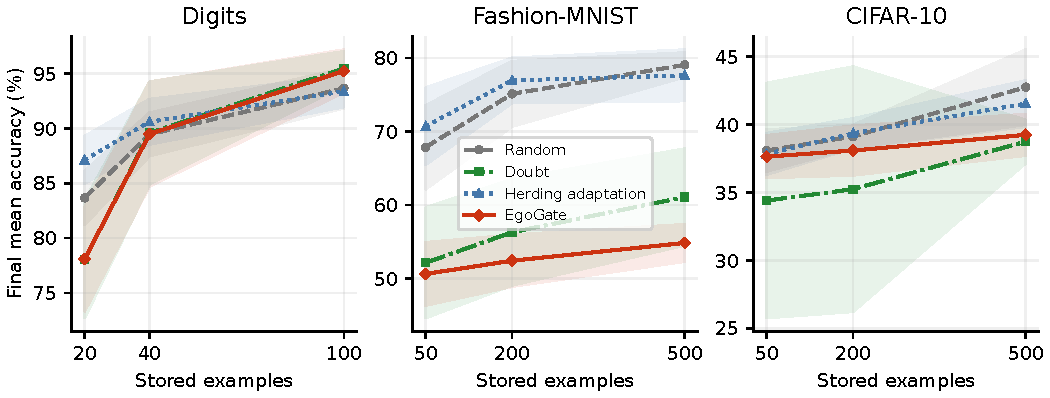
\includegraphics[width=\textwidth]{offline_benchmark.pdf}
\caption{Expanded offline benchmark across storage budgets. Lines show ten-seed means; shading shows one sample standard deviation, not a confidence interval. Primary significance tests use paired differences and Holm correction.}
\label{fig:expanded}
\end{figure*}

\subsection{Completed GPU Results}
All 870 runs completed on two Tesla T4 GPUs: 810 bounded-selector runs and
60 anchors. The audit verifies the complete grid, unique observations, matched
update/exposure counts, and selected-index hashes. Execution used Python
3.13.16, PyTorch 2.11.0+cu130, torchvision 0.26.0+cu130, CUDA 13.0,
NumPy 2.1.3, SciPy 1.16.3, and scikit-learn 1.6.1.

The expanded study does not establish a general advantage for EgoGate.
Across nine dataset/budget cells it has no significant wins over random,
Doubt, or herding after correction across the 27 primary tests. It has five
significant losses against random and five against herding: Digits at $K=20$,
all three Fashion-MNIST budgets, and CIFAR-10 at $K=500$. No comparison with
Doubt rejects after correction. Non-rejection is not evidence of equivalence.

At the central budgets (Table~\ref{tab:offlineexpanded}), Digits final accuracy
is 89.50\% for EgoGate and 89.47\% for random. Their paired difference is
$+0.03$ points, with a 95\% interval of $[-3.43,3.50]$. This differs from the
original fixed-split retention result. Randomized class partitions, data splits,
separated random generators, and the final-accuracy endpoint all change the
evaluation; the experiment does not isolate which change explains the discrepancy.

On Fashion-MNIST at $K=200$, EgoGate reaches 52.41\%, versus 75.11\% for
random and 76.94\% for herding. The EgoGate--random difference is $-22.70$
points (95\% interval $[-25.76,-19.64]$, Holm $p=1.02\times10^{-6}$).
Old-task accuracy is 15.92\% for EgoGate and 61.06\% for random, while
new-task accuracy is 88.90\% and 89.17\%, respectively. Thus the deficit
primarily concerns retention rather than a gain in new-task learning. EgoGate
still covers an average 4.9 of five old classes; counting represented classes
alone is insufficient to explain or prevent this failure.

CIFAR-10 exposes a severe limitation of the entire low-replay regime. At
$K=200$, random and EgoGate retain only 3.54\% and 1.73\% old-task accuracy,
despite 80.19\% mean accuracy before Task B. New-task accuracies are 74.72\%
and 74.45\%. Their final means, 39.13\% and 38.09\%, therefore conceal
near-complete old-task failure. The full-pool anchor reaches 52.25\% final
accuracy, which also falls short of strong continual learning. These results
must not be presented as competitive CIFAR performance or a comprehensive
comparison of modern continual-learning systems.

\subsection{Cost and Interpretation}
At CIFAR-10 $K=200$, mean EgoGate selection costs 10.48 s, versus less than
0.001 s for random and 0.88 s for herding. Task-B training takes about 25.3 s
for each. These synchronized timings exclude loading, base training, and final
evaluation; they quantify this implementation on the recorded hardware, not
universal latency. Equal update counts do not imply equal total compute.

The memory curves (Fig.~\ref{fig:expanded}) and complete secondary results
are supplied alongside all primary contrasts. A descriptive high mean for
EgoGate-diverse on Digits is not a confirmed primary-comparison win. Increasing
storage does not guarantee that global difficulty ranking becomes representative.
The study strengthens the evidence about the limits of the original selector;
it does not rescue its general-superiority claim. More replay, stronger
architectures, tuned optimization, and complete published baselines remain
necessary before drawing conclusions about broader continual-learning methods.


\section{From Learning Control to Agent Memory}
The architectural idea can also govern external memory for a deployed agent. Observations may include corrections, tool outcomes, or documents; retention may create a retrievable record rather than a weight update. A proposed implementation would retain provenance, distinguish authoritative updates from unverified statements, detect conflicting records, and support reversible consolidation. Its outcome measures would be future task success, repeated-error rate, stale-information use, review burden, and inference cost.

This is a separate application hypothesis. A hosted language-model interface ordinarily does not expose the parameter gradients required by (\ref{eq:gradient}). Replacing Curiosity with embedding novelty, answer disagreement, or a model judge changes the algorithm and needs independent validation. Improved context retrieval is not evidence of reduced catastrophic forgetting in model weights. Likewise, a tool interface can expose memory actions but cannot ensure that an agent invokes them for every observation; enforced admission requires integration into the memory-write path.

Chronological evaluation is necessary: a later correction must not appear in an earlier agent's context. Simple baselines include recency, deduplication, source-priority rules, and existing memory systems. The empirical question is whether adaptive admission yields additional future utility after all scoring and review costs.

\section{Limitations and Research Agenda}
\subsection{Selection Bias and Reliability}
Uncertainty and gradient magnitude can overselect noise. Confident errors can be rejected. Exploratory admission can reduce complete exclusion but cannot identify truth. Source verification, calibration under shift, rare-class coverage, and recovery after a misleading stream remain necessary experiments. No security guarantee follows from the quarantine metaphor.

\subsection{Adaptive Policies and Development}
The current selectors use fixed rules. An adaptive controller could learn coefficients or actions from delayed validation feedback, but obtaining unbiased feedback on rejected observations is itself difficult. Exploration, delayed labels, and counterfactual evaluation become part of the method. A contextual bandit may be suitable when decisions have limited downstream state effects; memory and parameter updates often have long-term consequences, making that simplification imperfect.

The personality hypothesis can be operationalized as persistent variation in learning behavior induced by experience. A suitable experiment would expose initially matched agents to environments of differing reliability, then test whether their learned policies transfer and remain correctable. Stable behavior alone is insufficient: a rigid gate may be consistent while performing poorly. No claim about subjective experience is implied.

\subsection{Generalization and Reproducibility}
Scaling requires stronger architectures, more diverse streams, delayed or absent labels, and total-resource comparisons. Both score parameterization and representation drift may alter ranking. The evaluated streaming extension deliberately sacrifices some sophistication for transparent implementation; it cannot substitute for comparisons with established methods. Archived results lack a contemporaneous environment manifest, whereas the new notebook records one. This difference must remain explicit when independent reproductions are compared.

\section{Conclusion}
Ego Gate frames continual learning as decisions about which experiences to retain, verify, learn, and consolidate. Its small offline replay result reproduces independently on Kaggle. The completed streaming study, however, shows that a direct heuristic extension can substantially underperform reservoir replay, and finds no statistically supported gain from the specified admission and periodic-consolidation changes. An unconditional exploratory replacement rule also imposes a severe retention bound.

The expanded 870-run offline study also fails to establish a general advantage: the combined selector has no significant primary-comparison wins and suffers substantial retention failures. The contribution is therefore a framework with narrow positive component evidence and documented limits in both expanded offline and online evaluations. Coverage preservation, reliable utility estimation, and controlled scheduling experiments are prerequisites for stronger claims. The present evidence does not validate an adaptive meta-controller, a commercial memory system, or a route to AGI.

\section*{Reproducibility}
Code and archived observations: \url{https://github.com/OptimistOtaku/ego-gate}. The companion package supplies the manuscript, raw observations, analysis, and private-execution notebook. The repository includes raw observations, source hashes, execution notebooks, tests, and analyses for all completed studies. The expanded benchmark contains 870 runs; the earlier Kaggle studies contain 380. These counts describe condition-seed runs, not independent datasets.

\section*{Acknowledgment}
OpenAI Codex assisted with all manuscript sections, experimental code, statistical analysis, and figure-generation code. The author must review the content and apply venue-specific disclosure requirements before submission. IEEE formatting does not imply peer review or acceptance.

\begin{thebibliography}{00}
\bibitem{ewc} J. Kirkpatrick et al., ``Overcoming catastrophic forgetting in neural networks,'' \emph{Proc. Natl. Acad. Sci.}, vol. 114, no. 13, pp. 3521--3526, 2017, doi: 10.1073/pnas.1611835114.
\bibitem{robins} A. Robins, ``Catastrophic forgetting, rehearsal and pseudorehearsal,'' \emph{Connection Science}, vol. 7, no. 2, pp. 123--146, 1995.
\bibitem{gss} R. Aljundi, M. Lin, B. Goujaud, and Y. Bengio, ``Gradient based sample selection for online continual learning,'' in \emph{Advances in Neural Information Processing Systems}, vol. 32, 2019.
\bibitem{mir} R. Aljundi et al., ``Online continual learning with maximally interfered retrieval,'' in \emph{Advances in Neural Information Processing Systems}, vol. 32, 2019.
\bibitem{gcr} R. Tiwari, K. Killamsetty, R. Iyer, and P. Shenoy, ``GCR: Gradient coreset based replay buffer selection for continual learning,'' in \emph{Proc. IEEE/CVF Conf. Computer Vision and Pattern Recognition}, 2022.
\bibitem{grasp} M. Y. Harun, J. Gallardo, J. Chen, and C. Kanan, ``GRASP: A rehearsal policy for efficient online continual learning,'' in \emph{Proc. Conf. Lifelong Learning Agents}, PMLR, vol. 274, pp. 1032--1052, 2025.
\bibitem{kendall} A. Kendall and Y. Gal, ``What uncertainties do we need in Bayesian deep learning for computer vision?'' in \emph{Advances in Neural Information Processing Systems}, vol. 30, 2017.
\bibitem{guo} C. Guo, G. Pleiss, Y. Sun, and K. Q. Weinberger, ``On calibration of modern neural networks,'' in \emph{Proc. Int. Conf. Machine Learning}, PMLR, vol. 70, pp. 1321--1330, 2017.
\bibitem{gal} Y. Gal and Z. Ghahramani, ``Dropout as a Bayesian approximation: Representing model uncertainty in deep learning,'' in \emph{Proc. Int. Conf. Machine Learning}, PMLR, vol. 48, pp. 1050--1059, 2016.
\bibitem{vime} R. Houthooft et al., ``VIME: Variational information maximizing exploration,'' in \emph{Advances in Neural Information Processing Systems}, vol. 29, pp. 1109--1117, 2016.
\bibitem{cls} J. L. McClelland, B. L. McNaughton, and R. C. O'Reilly, ``Why there are complementary learning systems in the hippocampus and neocortex: Insights from the successes and failures of connectionist models of learning and memory,'' \emph{Psychological Review}, vol. 102, no. 3, pp. 419--457, 1995.
\bibitem{collapse} I. Shumailov et al., ``The curse of recursion: Training on generated data makes models forget,'' arXiv:2305.17493, 2023.
\bibitem{amari} S. Amari, ``Natural gradient works efficiently in learning,'' \emph{Neural Computation}, vol. 10, no. 2, pp. 251--276, 1998.
\bibitem{digits} E. Alpaydin and C. Kaynak, ``Optical recognition of handwritten digits,'' UCI Machine Learning Repository, 1998, doi: 10.24432/C50P49.
\bibitem{sklearn} F. Pedregosa et al., ``Scikit-learn: Machine learning in Python,'' \emph{Journal of Machine Learning Research}, vol. 12, pp. 2825--2830, 2011.
\bibitem{holm} S. Holm, ``A simple sequentially rejective multiple test procedure,'' \emph{Scandinavian Journal of Statistics}, vol. 6, no. 2, pp. 65--70, 1979.
\bibitem{fashion} H. Xiao, K. Rasul, and R. Vollgraf, ``Fashion-MNIST: A novel image dataset for benchmarking machine learning algorithms,'' arXiv:1708.07747, 2017.
\bibitem{icarl} S.-A. Rebuffi, A. Kolesnikov, G. Sperl, and C. H. Lampert, ``iCaRL: Incremental classifier and representation learning,'' in \emph{Proc. IEEE Conf. Computer Vision and Pattern Recognition}, 2017, pp. 2001--2010.
\bibitem{cifar} A. Krizhevsky, ``Learning multiple layers of features from tiny images,'' University of Toronto, Tech. Rep., 2009.
\end{thebibliography}
\end{document}
